% CoRe-TFM JMLR working draft.
% Uses the official JMLR style file without modifying its layout.
% Compile with: latexmk -pdf main.tex
\documentclass[twoside,11pt]{article}
\usepackage[preprint]{jmlr2e}
\usepackage{amsmath,amsfonts,amssymb}
\usepackage{booktabs}
\hypersetup{hidelinks}

\newcommand{\TV}{\operatorname{TV}}
\newcommand{\KL}{\operatorname{KL}}
\newcommand{\E}{\mathbb{E}}
\newcommand{\Jone}{J^{B\rightarrow A}}
\newcommand{\Jtwo}{J^{A\rightarrow B}}
\newcommand{\Qhard}{Q_{\mathrm{hard}}}
\newcommand{\Qsoft}{Q_{\mathrm{soft}}}
\newcommand{\Cset}{\mathcal{C}}

\ShortHeadings{Selective Four-View Probability Reconciliation}{Anirudh}
\firstpageno{1}

\begin{document}

\title{CoRe-TFM: Selective Four-View Probability Reconciliation for Tabular Foundation Models}

\author{\name Badampudi Agasthya Anirudh \email anirudhbadampudi@gmail.com \\
       \addr Integrated M.Tech (Data Science)\\
       Institution and postal address to be completed\\
       India}

\maketitle

\begin{abstract}
Tabular foundation models (TFMs) can expose direct marginal and conditional probabilities that do not correspond to a common joint distribution. We study post-hoc reconciliation of four views, $p(A\mid X)$, $p(B\mid X)$, $p(A\mid B,X)$, and $p(B\mid A,X)$, without retraining the underlying model. Hard CoRe exactly preserves direct marginals; Soft CoRe relaxes marginal preservation through KL penalties; Selective CoRe uses held-out labels to choose among raw factorizations, pooling, and reconciliation. Known-truth experiments show that hard preservation helps when direct marginals are reliable and hurts when they are not. Across 100 heterogeneous controlled tasks, Selective CoRe beats arithmetic pooling by $0.00666$ mean NLL. The conclusion reverses in a bounded real-model benchmark covering ten data sets, five folds, and two TFMs: Selective CoRe is worse than arithmetic by $0.001831$ NLL (95\% bootstrap CI $[0.000548,0.003301]$; Wilcoxon $p=0.0273$), while reducing marginal distortion. Effects also reverse by model. These results establish probability reconciliation as a reliability-dependent consistency--accuracy trade-off and expose finite-validation selection as a principal deployment limitation.
\end{abstract}

\begin{keywords}
tabular foundation models, probabilistic consistency, probability reconciliation, proper scoring rules, information projection
\end{keywords}

\section{Introduction}
Tabular foundation models have rapidly become strong general-purpose predictors for structured data. TabPFN established that a transformer pretrained on synthetic tasks can perform competitive tabular prediction by in-context inference \citep{hollmann2025tabpfn}. More recent systems such as TabPFN-3 \citep{grinsztajn2026tabpfn3}, TabICLv2 \citep{qu2026tabiclv2}, and TabFM \citep{google2026tabfm} extend this paradigm in scale, speed, and task coverage. Their predictive probabilities are attractive not only for classification but also for uncertainty-sensitive decisions, conditional queries, sequential simulation, imputation, and multivariate scenario generation.

These uses expose a structural question that standard single-target benchmarks do not test. Suppose a frozen predictor is queried for two categorical targets $A$ and $B$. It can produce direct marginals $p(A\mid X)$ and $p(B\mid X)$, together with conditional predictions $p(A\mid B,X)$ and $p(B\mid A,X)$. If all four were views of one joint distribution, marginalization would recover the direct predictions and the two chain-rule factorizations would agree.

Recent work tested these requirements and found systematic marginalization and factorization violations across evaluated TFMs and datasets \citep{klotergens2026agree}. That result establishes a diagnosis: probabilities produced by the same frozen TFM need not be mutually representable by one joint. It does not determine the appropriate repair. Constructing any single normalized joint makes its own marginals and conditionals compatible by definition, so zero post-repair inconsistency is not evidence that the repaired probabilities are useful. A coherent distribution can have worse proper scores, worse calibration, or distorted dependence.

The distinction matters because recent TFM work increasingly evaluates the full predictive distribution. ScoringBench shows that model rankings depend on the proper scoring rule used \citep{landsgesell2026scoringbench}; conditional-density and uncertainty studies show strong predictive performance alongside reliability trade-offs \citep{izbicki2026cde,johnson2026uq}; and DistPFN demonstrates that targeted test-time posterior adjustment can improve a distinct failure mode, label shift, without retraining \citep{lee2026distpfn}. CoRe-TFM addresses neither generic calibration nor label shift. It addresses incompatibility among simultaneous probability views produced by the same predictor.

We formulate reconciliation as information projection over a finite categorical joint. The two autoregressive factorizations are treated as competing joint views. Arithmetic and geometric pooling provide principled KL-barycenter baselines. Hard CoRe projects a consensus distribution onto the transportation polytope defined by the two direct marginals. Soft CoRe relaxes exact marginal preservation with KL penalties and can be solved by generalized matrix scaling. Selective CoRe treats repair as a model-selection problem: validation data may select an original factorization, a simple pool, or a reconciliation policy.

The empirical design is diagnostic rather than winner-takes-all. First, a surrogate multiclass data-generating process provides exact $P^*(A,B\mid X)$ while finite-data estimators induce realistic coupled prediction errors. Second, an exact-view perturbation benchmark starts from the exact joint and independently perturbs the two marginals and two conditional families, isolating the reliability assumptions encoded by hard and soft reconciliation. Third, a heterogeneous task-mixture benchmark samples the reliability of all four views independently and evaluates whether Selective CoRe adapts to the task. A validation-size study measures how selection regret changes as held-out evidence grows.

Our contributions are:
\begin{enumerate}
\item a four-view formulation of TFM probability reconciliation that separates compatibility from calibration and predictive correctness;
\item Hard and Soft CoRe objectives, including a four-view KL decomposition and generalized Sinkhorn-style updates;
\item a Selective CoRe policy with a finite-candidate validation-selection guarantee;
\item an exact-view mechanism-identification benchmark showing when marginal preservation is beneficial or harmful;
\item a heterogeneous 100-task benchmark in which Selective CoRe significantly outperforms the best fixed method and remains close to a full candidate-family oracle;
\item a completed bounded-context benchmark over ten data sets, two released TFMs, a non-TFM boundary baseline, and five outer folds, showing that the full selector can lose to arithmetic pooling despite reducing marginal distortion;
\item a model-specific analysis revealing opposite Selective-CoRe effects for TabICLv2 and TabPFN-3; and
\item an auditable evaluation protocol with fold-level outputs, checksums, environment metadata, ablations, sensitivity analyses, and dataset-blocked inference.
\end{enumerate}

\section{Related Work}
\subsection{Tabular foundation models and probabilistic prediction}
TabPFN introduced prior-data fitted networks as pretrained Bayesian-like tabular predictors and demonstrated strong small-data performance \citep{hollmann2025tabpfn}. TabPFN-3 expands this approach to much larger tables and test-time compute scaling \citep{grinsztajn2026tabpfn3}. TabICLv2 provides an open, scalable in-context model with built-in handling of heterogeneous tabular features \citep{qu2026tabiclv2}. TabFM is another recent zero-shot TFM release \citep{google2026tabfm}. These systems differ in pretraining priors, scaling strategy, checkpoint access, and inference behavior, making a model-agnostic post-hoc consistency layer attractive.

Probability quality is now a first-class evaluation target. Proper-scoring benchmarks can reorder TFM conclusions \citep{landsgesell2026scoringbench}; conditional-density evaluation suggests that foundation models can be strong distributional predictors while still exhibiting calibration trade-offs \citep{izbicki2026cde}; and uncertainty studies emphasize that accurate means or classes need not imply reliable predictive uncertainty \citep{johnson2026uq}. DistPFN \citep{lee2026distpfn} is especially relevant as evidence that post-hoc probability adjustment for frozen TFMs can be useful, but it corrects label-shift bias rather than cross-query incompatibility.

\subsection{Consistency of conditional distributions}
The closest diagnostic work is \citet{klotergens2026agree}, which formalizes marginalization and factorization tests for TFMs. A broader theoretical precursor is \citet{majid2025consistent}, who study when families of learned conditional distributions can be recovered from a consistent joint and derive path, autoregressive, and swap consistency conditions. Compatibility of separately specified conditionals is older still; \citet{mure2017compromise} studies compromise distributions induced by incompatible conditionals. Conditioning consistency also appears in conditional neural processes \citep{young2026conditioning}. CoRe-TFM therefore does not claim to discover conditional inconsistency. Its narrower contribution is a post-hoc reconciliation family for the four views naturally exposed by frozen TFMs, evaluated by predictive fidelity rather than consistency alone.

\subsection{Joint tabular modeling as an alternative}
A different response to multivariate tabular inference is to train a model that represents a joint distribution directly. TabNAT learns order-agnostic conditional generation over mixed-type tables \citep{zhang2025tabnat}, while TabDiff uses a mixed-type diffusion process for joint generation and imputation \citep{shi2025tabdiff}. Such approaches avoid some composition problems by construction but require a generative training objective and model family. CoRe-TFM asks a complementary question: when a strong frozen discriminative TFM already exists, can its incompatible probability queries be reconciled after inference?

\subsection{Information projection and generalized scaling}
Hard reconciliation is an information projection onto a transportation polytope, closely related to iterative proportional fitting and Bregman projections \citep{benamou2015bregman}. Sinkhorn scaling is a central computational primitive for entropic transport \citep{cuturi2013sinkhorn}, and relaxed marginal constraints lead to generalized scaling updates \citep{chizat2018scaling}. We use these established tools as optimization machinery. Algorithmic novelty is not claimed for Sinkhorn scaling itself.

\section{Problem Formulation}
For a context data set $D$, test covariates $x$, and categorical targets $A\in\{1,\ldots,K_A\}$ and $B\in\{1,\ldots,K_B\}$, query the frozen predictor four ways:
\begin{align}
p_A(a)&=\hat p(A=a\mid x,D), & p_B(b)&=\hat p(B=b\mid x,D),\\
p_{A\mid B}(a\mid b)&=\hat p(A=a\mid B=b,x,D), &
p_{B\mid A}(b\mid a)&=\hat p(B=b\mid A=a,x,D).
\end{align}
These induce two normalized joints,
\begin{align}
\Jone(a,b)&=p_B(b)p_{A\mid B}(a\mid b),\\
\Jtwo(a,b)&=p_A(a)p_{B\mid A}(b\mid a).
\end{align}
A coherent system satisfies $\Jone=\Jtwo$. We measure factorization inconsistency by
\begin{equation}
\TV(\Jone,\Jtwo)=\frac12\sum_{a,b}|\Jone(a,b)-\Jtwo(a,b)|.
\end{equation}
Each direction also contains one non-trivial marginalization check because the first factor's marginal is satisfied by construction while the other need not match its direct prediction.

Our target is not merely any coherent $Q$. We seek a distribution that trades off agreement with $\Jone$ and $\Jtwo$, fidelity to $p_A$ and $p_B$, predictive scoring, and dependence preservation. On real data, the true posterior is unknown, so proper scores and calibration are primary. On controlled synthetic tasks, exact $P^*$ permits direct truth-distance evaluation.

\section{CoRe-TFM}
\subsection{KL-barycenter baselines}
For $w\in[0,1]$, define the arithmetic and geometric pools
\begin{align}
Q_{\mathrm{arith},w}&=w\Jone+(1-w)\Jtwo,\\
M_w(a,b)&=\frac{\Jone(a,b)^w\Jtwo(a,b)^{1-w}}{\sum_{a',b'}\Jone(a',b')^w\Jtwo(a',b')^{1-w}}.
\end{align}
The arithmetic pool minimizes $w\KL(\Jone\Vert Q)+(1-w)\KL(\Jtwo\Vert Q)$, whereas $M_w$ minimizes $w\KL(Q\Vert\Jone)+(1-w)\KL(Q\Vert\Jtwo)$. This makes both strong baselines rather than arbitrary averaging rules.

\subsection{Hard CoRe: marginal-preserving reconciliation}
Let
\begin{equation}
\mathcal{T}(p_A,p_B)=\left\{Q\ge0:\sum_bQ(a,b)=p_A(a),\;\sum_aQ(a,b)=p_B(b)\right\}.
\end{equation}
Hard CoRe is
\begin{equation}
\Qhard=\arg\min_{Q\in\mathcal{T}(p_A,p_B)}\KL(Q\Vert M_w).
\end{equation}

\begin{proposition}[Feasibility]
For any categorical marginals $p_A$ and $p_B$, $\mathcal{T}(p_A,p_B)$ is non-empty.
\end{proposition}
\begin{proof}
The independent joint $Q_0(a,b)=p_A(a)p_B(b)$ has exactly the required row and column sums.
\end{proof}

\begin{proposition}[Uniqueness under positive support]
If $M_w(a,b)>0$ for every cell, the Hard CoRe objective has a unique optimum on $\mathcal{T}(p_A,p_B)$.
\end{proposition}
\begin{proof}
The feasible set is convex and compact. $\KL(Q\Vert M_w)$ is strictly convex in $Q$ on the positive-support simplex, so a feasible minimizer exists and is unique.
\end{proof}

Iterative proportional fitting solves the finite problem by alternating row and column scaling. Hard CoRe changes dependence while exactly preserving the two direct marginals, which is useful only when those marginals deserve special trust.

\subsection{Soft CoRe: four-view reconciliation}
Hard marginal preservation can preserve a bad marginal. We therefore define
\begin{align}
\Qsoft=\arg\min_Q\;&w\KL(Q\Vert\Jone)+(1-w)\KL(Q\Vert\Jtwo)\nonumber\\
&+\lambda_A\KL(Q_A\Vert p_A)+\lambda_B\KL(Q_B\Vert p_B).
\label{eq:soft}
\end{align}
The first two terms equal $\KL(Q\Vert M_w)$ up to constants independent of $Q$. More importantly, the KL chain rule gives
\begin{align}
\KL(Q\Vert\Jone)&=\KL(Q_B\Vert p_B)+\E_{b\sim Q_B}\KL(Q_{A\mid B=b}\Vert p_{A\mid B=b}),\\
\KL(Q\Vert\Jtwo)&=\KL(Q_A\Vert p_A)+\E_{a\sim Q_A}\KL(Q_{B\mid A=a}\Vert p_{B\mid A=a}).
\end{align}
Thus Eq.~\eqref{eq:soft} is genuinely a four-view objective: both marginals and both conditional families influence the solution.

\subsection{Generalized matrix scaling}
For positive $M_w$, the optimum has scaling form $Q\propto\mathrm{diag}(u)M_w\mathrm{diag}(v)$. Let
\begin{equation}
\tau_A=\frac{\lambda_A}{1+\lambda_A},\qquad \tau_B=\frac{\lambda_B}{1+\lambda_B}.
\end{equation}
Alternating updates are
\begin{align}
u&\leftarrow\left(\frac{p_A}{M_wv}\right)^{\tau_A},\\
v&\leftarrow\left(\frac{p_B}{M_w^\top u}\right)^{\tau_B}.
\end{align}
These are generalized Sinkhorn-style updates for KL-relaxed marginals \citep{chizat2018scaling}. Our implementation retains an independent exponentiated-gradient solver and generic constrained optimizer on small instances as numerical cross-checks.

\subsection{Selective CoRe}
A single reconciliation strength cannot be optimal if view reliability changes by task. Selective CoRe therefore searches a finite policy family on an inner validation split. The current family contains the two original orders, arithmetic pooling, weighted geometric pooling, weighted Hard CoRe, and weighted Soft CoRe across five direction weights and seven marginal penalties, for 48 distinct candidates after removing duplicates. The chosen policy is then frozen and evaluated on held-out test data.

Let $L(Q)$ denote population joint log loss and $\hat L_v(Q)$ validation loss on $n_v$ independent examples. To make the selection guarantee finite, probabilities are floored at $\epsilon$ so loss is bounded by $B=-\log\epsilon$.

\begin{proposition}[Finite-candidate selection bound]
Let $\Cset$ contain $M$ candidate distributions and let $\hat Q=\arg\min_{Q\in\Cset}\hat L_v(Q)$. With probability at least $1-\delta$,
\begin{equation}
L(\hat Q)\le \min_{Q\in\Cset}L(Q)+2B\sqrt{\frac{\log(2M/\delta)}{2n_v}}.
\end{equation}
\end{proposition}
\begin{proof}
Hoeffding's inequality and a union bound give uniform deviation at most $c=B\sqrt{\log(2M/\delta)/(2n_v)}$ over $\Cset$. If $Q^*$ minimizes population loss in $\Cset$, then $L(\hat Q)\le\hat L_v(\hat Q)+c\le\hat L_v(Q^*)+c\le L(Q^*)+2c$.
\end{proof}
The bound is intentionally conservative because $B$ can be large, but it makes one qualitative prediction that we test directly: selection regret should decline with validation sample size.

\section{Experimental Design}
\subsection{Metrics and statistical principles}
Because the output is a probability distribution, proper scores are primary \citep{gneiting2007strictly}. We report joint NLL and Brier score; marginal NLL/Brier/accuracy; NLL and Brier for both conditionals induced by a candidate joint; factorization and marginalization TV; marginal and reconciliation distortion; mutual-information error; and runtime. Expected calibration error is retained as a descriptive diagnostic because it depends on binning and is not itself a proper scoring rule \citep{guo2017calibration}.

When exact $P^*(A,B\mid X)$ is known, we report exact expected log loss
\begin{equation}
\mathcal{L}_{P^*}(Q)=-\E_X\sum_{a,b}P^*(a,b\mid X)\log Q(a,b\mid X),
\end{equation}
plus TV and Jensen--Shannon distance to truth. Expected scores remove test-label Monte Carlo noise.

All adaptive decisions use validation labels disjoint from test observations. Paired effects are computed within random seed or task. Prespecified comparisons use two-sided Wilcoxon signed-rank tests; multiple comparisons within the exact-view regimes use Holm correction. Effect sizes accompany $p$-values.

\subsection{Surrogate DGP benchmark}
A multiclass DGP provides exact $P^*$. Gaussian features generate $A\mid X$ by softmax, while $B\mid A,X$ follows a second softmax with dependence parameter $\gamma$. Smooth nonlinear terms create misspecification for a multinomial logistic-regression surrogate. We vary one factor at a time: $\gamma\in\{0,0.5,1.5,3\}$; $n\in\{250,1000,5000\}$; $d\in\{5,20,50\}$; target cardinality in $\{2,3,5\}$; and three imbalance levels. Each condition uses 10 independent seeds.

\subsection{Exact-view perturbation benchmark}
The surrogate benchmark couples error across all four queries. We therefore start from exact $P^*$, derive compatible $p_A^*$, $p_B^*$, $p_{A\mid B}^*$, and $p_{B\mid A}^*$, and perturb each in log-probability space before renormalization. Six regimes are evaluated across 50 paired seeds: uniform low noise; reliable marginals; reliable conditionals; reliable $B\rightarrow A$ factorization; reliable $A\rightarrow B$ factorization; and uniformly high noise. This benchmark identifies which assumption makes a reconciliation method appropriate.

\subsection{Heterogeneous task-mixture benchmark}
To test Selective CoRe, we generate 100 independent tasks. On each task, the noise scale of each of the four views is drawn independently from a log-uniform distribution on $[0.04,0.75]$. Each task has 2,200 observations and a three-by-three target joint; 30\% of observations are used for validation and the remainder for exact expected test scoring. Selective CoRe searches the 48-candidate family described above. For analysis only, we also compute a non-deployable full-family oracle using exact test truth.

\subsection{Validation-size sensitivity}
A second mixture study uses 50 independently perturbed tasks with 3,200 observations each. A common test set is held fixed while selection is repeated with nested validation sizes $n_v\in\{100,250,500,800\}$. This directly evaluates the qualitative prediction of Proposition~3.

\section{Controlled Results}
\subsection{Coherence alone is insufficient}
The surrogate benchmark rejects a universal-ranking interpretation. At strong dependence ($\gamma=3$), Adaptive Soft CoRe obtains mean joint NLL 1.5854, compared with 1.6082 for arithmetic pooling and 1.6048 for Hard CoRe. A validation-selected original order obtains 1.5865, showing that adaptive repair is competitive but that selecting a reliable factorization can capture most of the available signal. The independent joint is much worse at 1.7435 despite being perfectly coherent and exactly preserving both direct marginals. Coherence is therefore a constraint, not an accuracy metric.

At $n=250$, arithmetic pooling is stronger than adaptive repair, while at larger sample sizes weighted pooling and selective policies become competitive. Raw inconsistency magnitude also fails as a universal repair trigger: across the dependence sweep, factorization TV has negligible rank association with Adaptive Soft's dividend over a validation-selected original order ($\rho\approx0.065$), but a stronger association with its advantage over unweighted arithmetic pooling ($\rho\approx0.422$, $p\approx0.0067$). Larger inconsistency can indicate that symmetric averaging is inadequate without proving that repair is better than trusting one order.

\subsection{Exact-view perturbations identify the reliability assumption}
Table~\ref{tab:exactview} and Fig.~\ref{fig:exactview} summarize the mechanism study. The best method changes exactly when the trust structure changes.

\begin{table}[t]
\caption{Best mean exact expected NLL in each exact-view perturbation regime (50 paired seeds).}
\label{tab:exactview}
\centering
\begin{tabular}{lll}
\toprule
Regime & Best method & Expected NLL\\
\midrule
Uniform low noise & Geometric pool & 1.478604\\
Direct marginals reliable & Soft CoRe ($\lambda=10$) & 1.486760\\
Conditionals reliable & Arithmetic pool & 1.508830\\
$B\rightarrow A$ reliable & $\Jone$ & 1.475308\\
$A\rightarrow B$ reliable & $\Jtwo$ & 1.475326\\
All four views noisy & Arithmetic pool & 1.538679\\
\bottomrule
\end{tabular}
\end{table}

\begin{figure}[t]
\centering
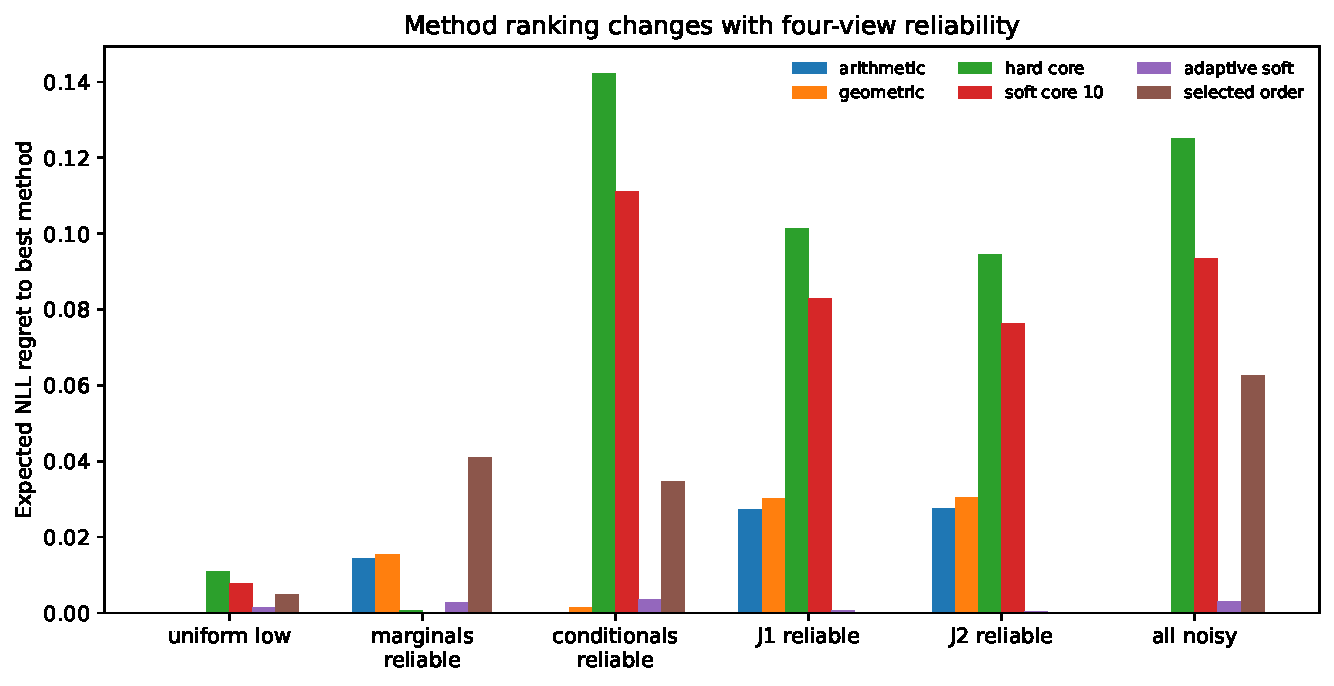
\includegraphics[width=0.98\textwidth]{Fig1_exact_view_regret.pdf}
\caption{Expected NLL regret to the best method in each exact-view reliability regime. Hard preservation is useful when direct marginals are reliable and costly when they are not.}
\label{fig:exactview}
\end{figure}

When direct marginals are reliable and conditionals are noisy, Hard CoRe improves over arithmetic pooling by 0.01327 NLL on average; the Holm-adjusted paired Wilcoxon $p$-value is $7.11\times10^{-15}$. Strong Soft CoRe is slightly better still. When direct marginals are noisy and conditionals reliable, the conclusion reverses: Hard CoRe is worse than arithmetic by 0.15048 NLL on average ($p_{\mathrm{Holm}}=7.11\times10^{-15}$). Adaptive Soft is 0.14660 better than Hard CoRe but remains 0.00388 worse than arithmetic. Exact marginal preservation can therefore amplify a bad marginal forecast.

Directional regimes provide a third sanity check. When the $B\rightarrow A$ factorization is reliable, $\Jone$ is best and Adaptive Soft is only 0.00054 NLL worse than the validation-selected order. The analogous pattern holds for $\Jtwo$. Under symmetric low or high noise, arithmetic/geometric pooling is difficult to beat. A reconciliation algorithm cannot create information absent from its inputs, so a correct deployment policy must be able to retain a trustworthy direction or simple pool.

\subsection{Selective CoRe adapts across heterogeneous tasks}
The heterogeneous task-mixture study is the strongest controlled test of Selective CoRe. Table~\ref{tab:mixture} reports exact expected NLL over 100 tasks. Selective CoRe has the best mean score among deployable methods, 1.48368, compared with 1.49034 for the best fixed method, arithmetic pooling. The paired difference is $-0.00666$ NLL; Selective CoRe wins on 68/100 tasks and the Wilcoxon $p$-value is $1.25\times10^{-11}$.

\begin{table}[t]
\caption{Heterogeneous 100-task mixture benchmark. Oracle regret is measured against the same full 48-candidate family available to selection, evaluated with exact test truth only for analysis.}
\label{tab:mixture}
\centering
\begin{tabular}{lrrr}
\toprule
Method & Mean NLL & SE & Mean full-oracle regret\\
\midrule
Selective CoRe & \textbf{1.483684} & 0.005470 & \textbf{0.000710}\\
Arithmetic & 1.490344 & 0.005553 & 0.007370\\
Geometric & 1.491382 & 0.005584 & 0.008408\\
Soft CoRe ($\lambda=1$) & 1.500597 & 0.005997 & 0.017623\\
$\Jtwo$ & 1.506846 & 0.006989 & 0.023872\\
$\Jone$ & 1.514449 & 0.006691 & 0.031475\\
Hard CoRe & 1.538343 & 0.008471 & 0.055369\\
\bottomrule
\end{tabular}
\end{table}

The policy does not collapse to one candidate. Across 100 tasks it selects Soft CoRe 38 times, geometric pooling 33 times, an unrepaired original order 19 times, and arithmetic pooling 10 times; Hard CoRe is never selected. This diversity is expected under independently sampled view reliability. Fig.~\ref{fig:mixture} shows the paired task-level gain over arithmetic pooling.

\begin{figure}[t]
\centering
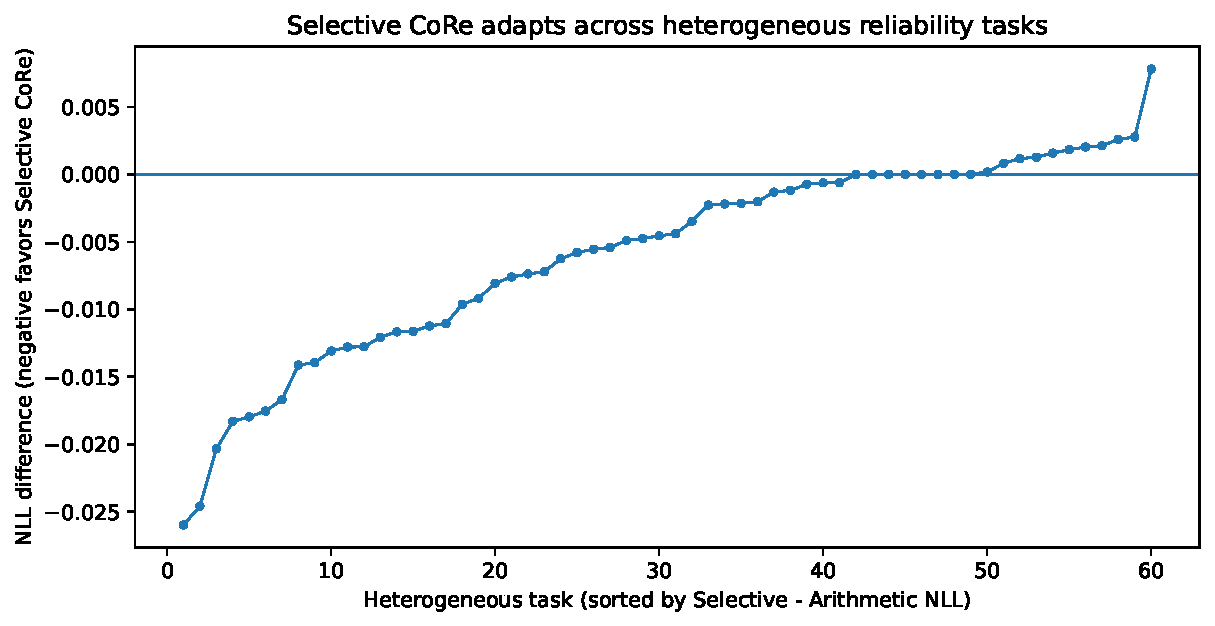
\includegraphics[width=0.92\textwidth]{Fig2_selective_task_gain.pdf}
\caption{Task-level difference in exact expected NLL between Selective CoRe and arithmetic pooling, sorted across the 100 heterogeneous reliability tasks. Negative values favor Selective CoRe.}
\label{fig:mixture}
\end{figure}

\subsection{More validation data reduces selection regret}
The controlled validation-size study supports the finite-candidate analysis. Mean regret to the full candidate-family oracle falls monotonically from 0.00560 at 100 validation observations to 0.00115 at 800 (Table~\ref{tab:valsize}). The mean gain over arithmetic grows from 0.00067 to 0.00512. The finite-sample bound is not numerically tight, but its $n_v^{-1/2}$ dependence captures the observed controlled-task direction.

\begin{table}[t]
\caption{Validation-size sensitivity across 50 heterogeneous tasks.}
\label{tab:valsize}
\centering
\begin{tabular}{rrrr}
\toprule
$n_v$ & Mean Selective NLL & Mean oracle regret & Mean gain over arithmetic\\
\midrule
100 & 1.486995 & 0.005602 & 0.000670\\
250 & 1.483853 & 0.002460 & 0.003813\\
500 & 1.483083 & 0.001690 & 0.004583\\
800 & 1.482548 & 0.001155 & 0.005118\\
\bottomrule
\end{tabular}
\end{table}

\begin{figure}[t]
\centering
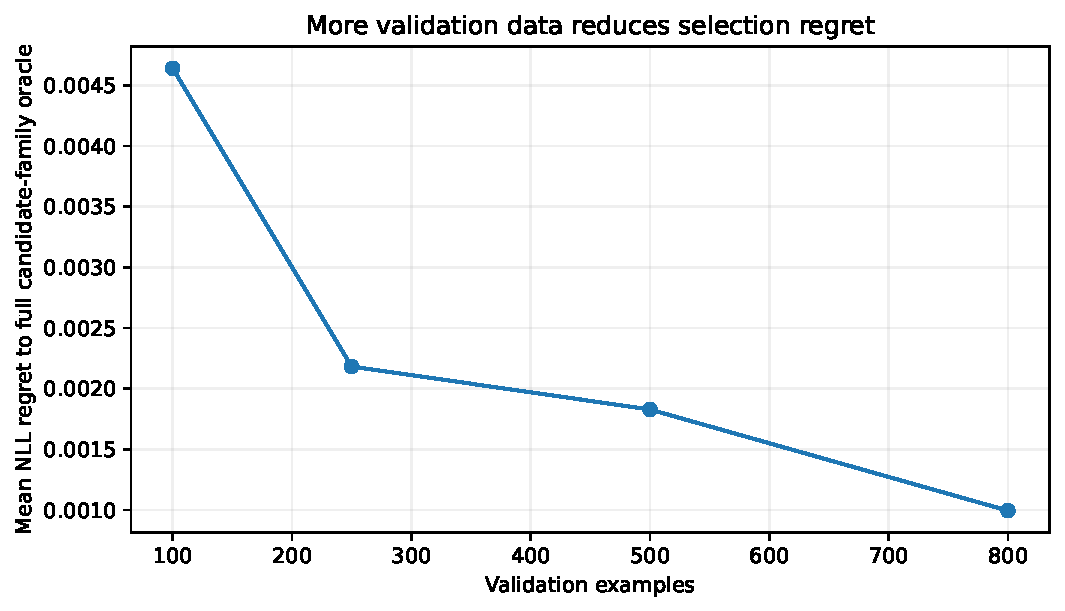
\includegraphics[width=0.78\textwidth]{Fig3_validation_size.pdf}
\caption{Mean exact NLL regret of Selective CoRe to the full candidate-family oracle as validation sample size increases.}
\label{fig:valsize}
\end{figure}

\subsection{Directional defects are not correctness signals}
A natural label-free heuristic is to trust the factorization whose implied missing marginal is closer to its direct prediction. We tested this rule in the surrogate DGP. Direction-selection accuracy weakens toward or below chance as dependence increases. We retain this as a negative ablation: a small internal consistency defect is not evidence that a factorization is closer to $P^*$.

\subsection{Computational overhead}
On a local batch of 5,000 $5\times5$ joints, generalized scaling reaches the same soft objective as an independent exponentiated-gradient solver while requiring approximately 0.022 seconds versus 0.101 seconds. The intended interpretation is practical: reconciliation is lightweight relative to TFM inference. We do not claim optimization novelty over generalized Sinkhorn methods.

\section{Bounded Real-Model Benchmark}
The real-model study evaluates Anneal, Car, Credit, Customer, Diamonds, Marketing, MIC, Nursery, Phishing, and Wine. Each of five deterministic outer folds uses a class-covering sample of at most 256 training observations, 52 disjoint validation observations, and 128 test observations. The primary TFM models are TabICLv2 2.1.1 (two estimators, no key--value cache) and TabPFN 8.4.0 using its TabPFN-3 interface. CatBoost 1.2.10 is included only as a non-TFM boundary baseline. TabFM was excluded before comparative scores were inspected because its released implementation was operationally incompatible with the bounded Colab protocol and prohibitively slow. CatBoost is not counted as its replacement in TFM claims.

Every dataset--model--fold task fits the four views on the outer training sample. A fixed 20\% inner split selects among 48 raw, pooled, hard, and soft candidates; the policy is then frozen before scoring the outer test sample. The completed matrix contains 150 fold tasks and 1,200 method rows. Package versions, hardware, data hashes, fold manifests, and SHA-256 checksums are archived. Because training and test contexts are bounded, these results answer a small-context question and are not directly comparable to the earlier full-training Car and Wine pilots.

\subsection{Primary dataset-blocked comparison}
The inferential unit is the dataset. For each method and dataset we first average five folds within each TFM and then average TabICLv2 and TabPFN-3. CatBoost is excluded. The prespecified contrast is Selective CoRe minus equal-weight arithmetic pooling, so negative values favor Selective CoRe.

\begin{table}[t]
\centering
\caption{Dataset-blocked Selective-CoRe effects relative to arithmetic pooling across the two primary TFMs ($n=10$ datasets). Confidence intervals resample datasets; $p$-values are two-sided paired Wilcoxon tests.}
\label{tab:realprimary}
\begin{tabular}{lrrrr}
\toprule
Metric & Mean difference & 95\% bootstrap CI & Wins & $p$ \\
\midrule
Joint NLL & $+0.001831$ & $[+0.000548,+0.003301]$ & 2/10 & 0.02734 \\
Joint Brier & $+0.000646$ & $[+0.000288,+0.001059]$ & 1/10 & 0.00586 \\
ECE (15 bins) & $+0.000096$ & $[-0.002706,+0.003017]$ & 6/10 & 1.00000 \\
Marginal distortion & $-0.003855$ & $[-0.005563,-0.002212]$ & 9/10 & 0.00391 \\
\bottomrule
\end{tabular}
\end{table}

Selective CoRe therefore improves agreement with the direct marginals but worsens both proper scores. Its joint-NLL disadvantage is positive in eight of ten datasets and remains positive under every leave-one-dataset-out mean. Mean factorization TV is 0.06249 across the 20 primary TFM cells, confirming that the probability views are genuinely incompatible; incompatibility alone nevertheless does not justify a more complex selector.

\begin{figure}[t]
\centering
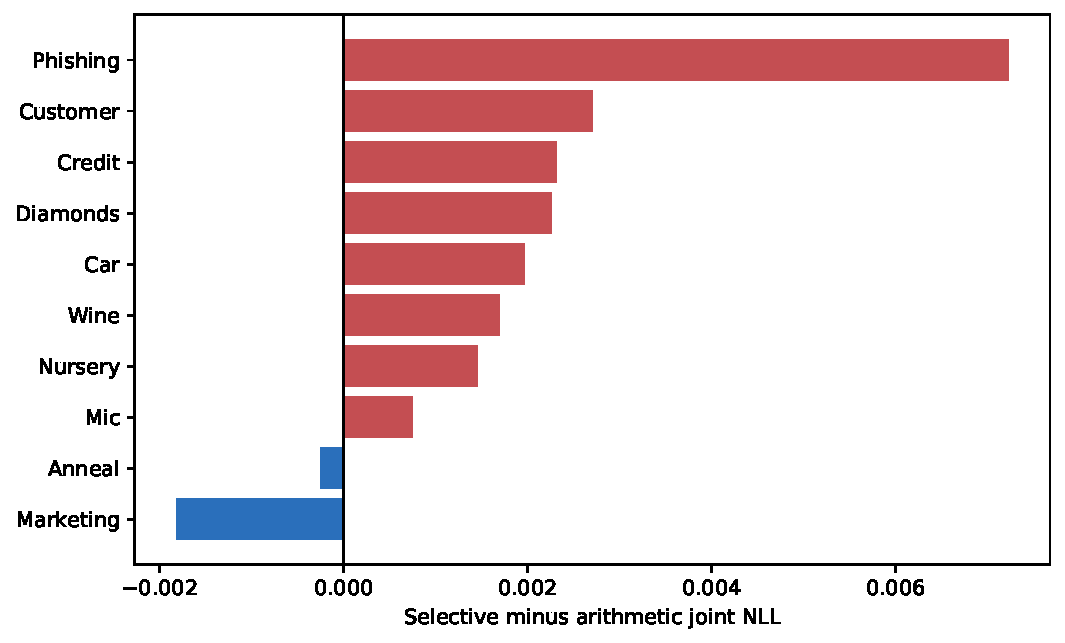
\includegraphics[width=0.78\textwidth]{Fig4_real_dataset_effects.pdf}
\caption{Dataset-blocked joint-NLL effect of Selective CoRe relative to arithmetic pooling after averaging TabICLv2 and TabPFN-3. Negative values favor Selective CoRe.}
\label{fig:realeffects}
\end{figure}

\subsection{Model heterogeneity and consistency tax}
The average effect reverses by model. Selective CoRe is worse than arithmetic by 0.006694 NLL on TabICLv2 (2/10 wins), but better by 0.003031 on TabPFN-3 (5/10 wins). The paired difference between these model-specific effects is 0.009725 ($p=0.00977$; exploratory). CatBoost's descriptive effect is $+0.001771$ with 4/10 wins. Thus averaging models conceals a reproducible interaction between the upstream predictor and the value of validation-based reconciliation.

Hard CoRe nearly eliminates marginal distortion but is worse than arithmetic by 0.02056 NLL on every primary dataset ($p=0.00195$). The independent joint is also exactly marginal-preserving and worse by 0.13674 NLL. Geometric pooling is descriptively 0.000492 better than arithmetic, but the paired comparison is not significant ($p=0.7695$). These results separate mathematical coherence from probabilistic accuracy.

\subsection{Selection-family and validation-size ablations}
Restricting the selector to pooling candidates gives mean NLL 1.375591 across all 30 active cells, compared with 1.376046 for the full family, 1.376390 for repair-only selection, and 1.378435 for raw-only selection. The full candidate family therefore pays a small selection cost. The real-data validation-fraction analysis is non-monotone: using 25\%, 50\%, and 100\% of the fixed 52-example pool gives mean NLL 1.375074, 1.376495, and 1.376046, respectively. Unlike the controlled validation-size experiment, this bounded real study does not establish monotonic improvement with more labels.

\section{Discussion}
\subsection{Coherence, calibration, and correctness are different properties}
Compatibility asks whether multiple probability queries can be represented by one joint. Calibration asks whether stated probabilities match empirical frequencies. Proper scoring evaluates the complete predictive distribution. Distance to $P^*$ asks whether a controlled posterior is recovered. The experiments show that these properties can disagree. The independent baseline is coherent and can be poor; Hard CoRe can preserve two accurate marginals or two inaccurate marginals with equal mathematical success; and a reliable raw factorization can outperform a more coherent repair.

\subsection{Marginal penalties have a reliability interpretation}
The exact-view study gives $\lambda$ a statistical meaning. Large $\lambda$ expresses trust in direct marginals, while small $\lambda$ allows conditional evidence to move them. The best penalty is therefore not merely a numerical tuning constant. It is a task-specific estimate of relative reliability among four model queries.

\subsection{Selection is useful only with enough evidence}
Released TFMs differ in pretraining prior, architecture, scale, and inference strategy. The model-specific sign reversal confirms that relative reliability of direct and conditional queries changes in practice. Keeping raw factorizations and pools inside the candidate family is therefore necessary, but not sufficient: the bounded study shows that searching 48 candidates with 52 validation labels can lose to arithmetic pooling. Selective CoRe should be understood as an option whose complexity must be matched to validation information, not as a universally preferred endpoint.

\subsection{Relation to joint generative models}
Joint tabular generators such as TabNAT and TabDiff avoid some composition problems by directly modeling mixed-type joint distributions \citep{zhang2025tabnat,shi2025tabdiff}. That is a compelling alternative when retraining or a generative model is feasible. CoRe-TFM instead targets the increasingly common case in which a high-performing frozen discriminative TFM already exists and multiple conditional queries are assembled downstream.

\section{Limitations and Threats to Validity}
First, the current formulation is pairwise and categorical. Global consistency across many targets introduces additional compatibility constraints and potentially exponential state spaces. Second, regression and mixed discrete--continuous targets are deferred. Third, the real benchmark uses only two TFMs; CatBoost is a boundary baseline rather than a third foundation model. Fourth, all primary folds use one deterministic constrained sample with at most 256 training observations. Independent sampling seeds and larger context sizes are needed to determine whether the model interaction persists. Fifth, Marketing and Nursery contain extremely rare target classes, so a rare-class exclusion sensitivity is required. Sixth, the 48-candidate selector is large relative to its 52-example validation set and demonstrably incurs selection cost. Seventh, ECE is descriptive; conclusions rely primarily on proper scores. Finally, the controlled task mixture is a designed stress test, not an estimate of the natural frequency of view-reliability regimes in deployed TFMs.

\section{Reproducibility}
The repository contains the exact 33-cell Colab notebook, 1,200 fold-level result rows, controlled replications, ablations, validation sensitivity, fold manifests, source and data hashes, package versions, hardware metadata, plots, and a checksum manifest. A repository-native audit command validates the matrix and regenerates dataset-blocked effects. The archived run used Python 3.13.15, PyTorch 2.11.0 with CUDA 12.8, TabICL 2.1.1, TabPFN 8.4.0, CatBoost 1.2.10, and a Tesla T4. The source snapshot recorded by the run is commit \texttt{3c32c02}; the current repository adds the evidence and manuscript updates without representing them as part of that earlier execution snapshot. TabPFN access credentials are never stored.

\section{Conclusion}
CoRe-TFM reframes probability consistency as a four-view reliability problem rather than a projection problem with a universal answer. Controlled experiments establish the mechanism: marginal preservation helps only when the marginals deserve trust, and Selective CoRe can adapt when validation evidence is abundant. The bounded real-model result adds the necessary counterweight. Across ten datasets, Selective CoRe reduces marginal distortion but is significantly worse than arithmetic pooling on NLL and Brier score; its effect reverses between TabICLv2 and TabPFN-3, and pool-only selection beats the full family. The defensible conclusion is therefore conditional: reconcile when the reliability structure and validation budget support it, and otherwise retain a strong simple pool. Independent sampling seeds, context-size sensitivity, rare-class robustness, and preferably a third released TFM remain necessary before submission.

\acks{Funding and competing-interest disclosures will be completed before submission. No external funding has been declared in this working draft. The author remains responsible for verifying all experimental results, code, claims, citations, and the final manuscript.}

\appendix
\section{Additional Derivations}
\subsection{Why arithmetic and geometric pools are KL barycenters}
For normalized distributions $P_1$ and $P_2$, minimizing $w\KL(P_1\Vert Q)+(1-w)\KL(P_2\Vert Q)$ over normalized $Q$ is equivalent to maximizing $\sum_z[wP_1(z)+(1-w)P_2(z)]\log Q(z)$, giving the arithmetic pool. Reversing the KL arguments yields an objective whose $Q$-dependent part is $\sum_z Q(z)\log Q(z)-\sum_zQ(z)[w\log P_1(z)+(1-w)\log P_2(z)]$, whose normalized minimizer is the weighted geometric pool.

\subsection{Four-view decomposition}
For $\Jone(a,b)=p_B(b)p_{A\mid B}(a\mid b)$,
\begin{align}
\KL(Q\Vert\Jone)
&=\sum_{a,b}Q(a,b)\log\frac{Q_B(b)Q_{A\mid B}(a\mid b)}{p_B(b)p_{A\mid B}(a\mid b)}\\
&=\KL(Q_B\Vert p_B)+\E_{b\sim Q_B}\KL(Q_{A\mid B=b}\Vert p_{A\mid B=b}).
\end{align}
The $\Jtwo$ decomposition is symmetric. This identity is what makes Soft CoRe a four-view rather than two-matrix objective.

\section{Exact-View Perturbation Details}
For each exact probability vector $p$, perturbation is performed in log space,
\begin{equation}
\tilde p_i=\frac{\exp(\log p_i+\sigma\epsilon_i)}{\sum_j\exp(\log p_j+\sigma\epsilon_j)},\qquad \epsilon_i\sim\mathcal{N}(0,1).
\end{equation}
The four view-specific $\sigma$ values define the reliability regime. This preserves positivity and normalization while allowing marginal and conditional errors to be controlled independently.

The prespecified paired comparisons per regime are Hard CoRe versus arithmetic, Adaptive Soft versus arithmetic, Adaptive Soft versus Hard CoRe, and Adaptive Soft versus validation-selected original order. Holm correction is applied within each regime. The most important sign reversal is Hard minus arithmetic: $-0.013270$ when marginals are reliable, but $+0.150481$ when conditionals are reliable and marginals are noisy; both adjusted $p$-values are $7.11\times10^{-15}$.

\section{Selective Candidate Family}
The selector includes two original orders, arithmetic pooling, weighted geometric pooling, weighted Hard CoRe, and weighted Soft CoRe. Direction weights are $\{0,0.25,0.5,0.75,1\}$ and soft marginal penalties are $\{0.03,0.1,0.3,1,3,10,30\}$. Duplicate half-weight geometric and hard candidates are removed, leaving 48 candidates. Ties prefer lower-complexity policies and less-extreme hyperparameters. The full-family oracle in Sec.~7.3 evaluates exactly this same set using test truth and is never used for deployment or hyperparameter selection.

\section{Real-TFM Reporting Checklist}
For each model--data set cell, the release reports factorization TV, joint NLL/Brier/ECE, induced conditional NLLs, marginal distortion, selected policy/hyperparameters, fold-level values, package versions, hardware, and provenance. Primary cross-model conclusions use datasets after averaging the two TFMs; the 30-cell table is descriptive only and must not be labeled confirmatory. Future extensions should additionally record solver iterations and convergence residuals and should use a frozen hierarchical or paired dataset-blocked analysis.

\bibliography{references}
\end{document}
